\chapter{Background} % Background

% proposal
\label{ch:background}
In this chapter we present basic concepts that are needed to understand better
our work. In \autoref{sec:switchedsystems} we define some definitions about switched systems 
and the difference between hybrid system a basic concept that we will use for our
analysis,

% \ref{} to equations or tables

\clearpage

% commments: aun no me queda claro sonbre la ecuacion de distribucion del uncontrollable event

\section{Switched systems}
\label{sec:switchedsystems}
    \textbf{Switched systems} are loosely defined as dynamical system whose state has
    two components, one of which evolves in a continuous set such as 
    $\mathbb{R}$  while the other evolves in a discrete set such as
    $\mathbb{N}$ according to some transition logic based rule. 
    Hybrid System is an bastract meaning of switched system which 
    is a system which changes acording to switch rule, this rule 
    comprises of discrete events, \citep{branicky1994stability}.

    \begin{figure}[!h]
        \begin{center}
            \includegraphics[width=\textwidth*4/5]{images/ss}
            \caption{atched System Schematic}
        \end{center}
    \end{figure}

    Let us consider nonlinear switched systems such that

    \begin{equation}
        \dot x = f_{\sigma(t)}(x(t),d(t)) \\
    \end{equation}

    defined for all $t \geqslant 0$, where $x(t) \in \mathbb{R}^n$ is the state
    of the system, $\sigma(.): \mathbb{R}^+ \rightarrow U$ is the switching 
    rule, and $d(t) \in \mathbb{R}^m$ is a bounded perturbation. The finite
    set $U = \left\lbrace 1,2,.. N \right\rbrace$ is the set of switching
    modes of the system. We focus on sampled switched systems: given a sampling
    period $\tau > 0$, switching will occur at time $\tau, 2\tau, ...$ Switching 
    depend only on time, and not on states: \emph{this is the main difference with 
    hybrid system}.

    We work in the \emph{synchronous} setting for discrete events. This means
    that all the discrete events are supposed to occur at periodic instants:
    $\tau, 2\tau, 3\tau, ...$ The switching rule $\sigma(.)$ is thus piecewise
    constant, we shall consider that $\sigma(.)$ is constant on the time interval
    $[(k-1)\tau,k\tau[$ for $k \geqslant 1 $. We call \emph{"pattern"} a finite
    sequence of modes $\pi =  (i_1,i_2,...i_k) \in U^k$. With such a control
    input, and under a given perturbation $d$, we shall denote by $x(t;t_0;x_0,d,\pi)$
    the solution at time $t$ of the system.
    
    \begin{equation} % move to center then
        \begin{array}{l}
            \dot x (t) = f_{\sigma(t)}(x(t),d(t)), \\
            x(t_0) = x_0, \\
            \forall j \in \left\lbrace 1, ... , k \right\rbrace, \sigma(t)=i_j
            \in U \text{ for, } t \in \lbrack 1,2 \lbrack
        \end{array}
        \label{hybridsystem}
    \end{equation}

    % We address the "problem" of synthesizing a state-dependent switching rule
    % $\sigma(.)$ for \ref*{hybridsystem} in order to verify some properties.
    % This important problem is formalized as follows.

    We will use \ref{hybridsystem} in order to have a clear understanding about
    some definitions that will be useful for our methodology.

    \begin{figure}[!h]
        \begin{center}
            \includegraphics[width=\textwidth*3/5]{images/swiched}
            \caption{Trajectory of a hybrid system. The switching signal
            ${\sigma(t)}$ takes on integer values that change at 
            discrete-time instances.\citep{liberzon2003switching}}
        \end{center}
    \end{figure}



\section{Safe patterns computation}
\label{sec:safepatterncomputation}
    In this part is presented a some definitions based on an existing 
    procedure of state-space bisection and made available for nonlinear 
    systems  with the help of guaranteed integration, the algorithm has
    been  improved to be able to consider longer patterns of modes with a better
    pruning approach. The method consist of given a objective region 
    \emph{R}, a set \emph{S} and a forbidden reigion \emph{B}, the method find a pattern $\pi_i$, $i \in 
    \mathbb{N}$. \cite{le2016distributed}, some definitions are shows as follow:

    \textbf{Definition 1} \emph{((R,S) - Stability Problem)}. Given a 
    switched system as shown in figure before, a set of recurrence 
    ${\mathbb{R}^n}$ and a safe set \emph{S}
    ${\subset \mathbb{R}^n}$,\textbf{there are} a control rule 
    ${\sigma : \mathbb{R}^+ \rightarrow U}$ such that, for any
    initial condition ${x_0  \in  R_1}$ and any perturbation 
    ${\varpi :\mathbb{R}^+\rightarrow U}$  the
    following holds:
    
    \begin{itemize}
        \item \emph{ Recurrence in \emph{R}: There are a monotonically 
        strictly increasing sequence of (positive) integers
        ${\lbrace k_l \rbrace_{l \in \mathbb{N}} , t \in \mathbb{N}}$ such 
        that for all ${ l \in \mathbb{N}, \phi(k_l\tau;t_0,x^0,\sigma,w) \in R }$.}
        \item \emph{ Stability in \emph{S}: For all ${ t \in \mathbb{R}^n,
        \phi(t;t_0,x^0,\sigma,w) \in S}$ .}
    \end{itemize}
    
    \textbf{Definition 2} \emph{((${R_1,R_2,S}$) - Reachability ). %problem
        Given a switched system of the form shown above, two sets  
        ${ R_1 \subset \mathbb{R}^n}$  and ${ R_2 \subset \mathbb{R}^n}$ 
        and a safety set  ${S \subset  \mathbb{R}^n}$, $R_2$ is reachable if
        %find a 
        there is a control rule  ${\sigma}$ :
        ${\mathbb{R}^+\rightarrow U}$ such that, for any initial condition 
        ${x_0  \in  R_1}$ and any perturbation  ${\varpi : \mathbb{R}^+  
        \rightarrow U}$, the following holds:}
    
    \begin{itemize}
        \item  \emph{Reachability from ${R_1}$ to ${R_2}$: there exists 
        an integer ${k \in \mathbb{N} }$ such that we have ${ \phi( k_l\tau
        ;t_0,x^0,\sigma,w) \in R_2 }$.}
        \item \emph{ Stability in S: for all ${ t \in \mathbb{R}^+, 
        \phi(t;t_0,x^0,\sigma,w) \in S}$ .}
    \end{itemize}
    
    \textbf{Definition 3}\emph{(Safe Control Synthesis)}. Let us 
    consider a sampled switched system. Given three sets R, S and B, 
    with ${R \cup B \in S}$  and ${R \cap B = \varnothing }$. % find a 
    The system is safe if there is a rule ${\sigma(.)}$ such that, 
    for any ${x(0) \in R }$. 

    \begin{itemize}
        \item \emph{ ${\tau}$-stability: ${x(t)}$ return in R 
        infinitely often, at some multiples of sampling time ${\tau}$}.
        \item \emph{ safety: ${x(t)}$ always stays in ${S/B}$.}
    \end{itemize}

    \begin{algorithm}    
        \caption{Decomposition}\label{decomposition}    
        \begin{algorithmic}[1]
          \Procedure{Decomposition}{$W,R,S,B,D,K$}\Comment{List of set of patterns} \\
            \textbf{Input:} A box $W$, a box $R$, 
            a box $S$, a box $B$, a degree $D$ of bisection, a length $K$ of input pattern\\
            \textbf{Output:} $ \lbrace(V_i,\pi_i)\rbrace_i, True $ or $ <_,False>$ \\          
            $(\pi,b) := FindPattern(W,R,S,B,K)$
            \If{ $b = True$}
              \State return $<\lbrace (W,pat) \rbrace,True>$
            \Else
              \If{ $D = 0$}
                \State return $<,False>$
              \Else
                \State Divide equally $W$ into $(W_1,W_2)$
                \For{ $i=1,2$}
                  \State $(,b_i) = Decomposition(W,R,SB,D-1,K)$
                \EndFor
              \EndIf
            \EndIf
            \State \textbf{return} $<_,False>$.
          \EndProcedure    
        \end{algorithmic}
      \end{algorithm}


      \begin{algorithm}
        \caption{Find Pattern with forbidden transitions}\label{findPattern}
        \begin{algorithmic}[1]
          \Procedure{FindPattern}{$W,R,S,B,K$}\Comment{List of set of patterns} \\
            \textbf{Input:} A box $W$, a box $R$,
            a box $S$, a box $B$, a length $K$ of input pattern\\
            \textbf{Output:} $<\prod,True> or <_,False>$ \\
            $\mathcal{S}= \lbrace \emptyset \rbrace$ \\
            $\mathcal{L}= \lbrace (W,W,\emptyset) \rbrace$
            \While{$\mathcal{L} \neq \emptyset$}
              \State $e_{current} = takeHead(\mathcal{L})$
              \For{$i \in U$}:
                \If {$Pair(l,i) = False $}\Comment{$l$ is the current mode}
                  \State \textbf{continue}\Comment{Not considered transition $l,i$}
                \EndIf                
                \If {$ Post_{i}(e_{current}.Y_{current}) \subseteq R$ \textbf{and} $Tube_{i}(e_{current}.Y_{current}) \cup B = \emptyset $ \textbf{and} $Tube_{i}(e_{current}.Y_{current}) \cup B \subseteq S $ }
                  \State putTail($\mathcal{S}e_{current}.\prod + i$)
                \Else
                  \If{$ Tube_{i}(e_{current}.Y_{current}) \cap B \neq \emptyset $ \textbf{or} $ Tube_{i}(e_{current}.Y_{current}) \nsubseteq S $}
                    \State discard $e_{current}$
                  \EndIf
                  \If{$ Tube_{i}(e_{current}.Y_{current}) \cap B = \emptyset $ \textbf{and} $ Tube_{i}(e_{current}.Y_{current}) \subseteq S $}
                    \If {$Length(\prod)+1<K$}
                      \State putTail$(\mathcal{L},(e_{current}.Y_{init}.Post_{i}(e_{current}.Y_{current}),e_{current}.\prod+i))$
                    \EndIf              
                  \EndIf
                \EndIf
              \EndFor          
            \EndWhile
            \State \textbf{return} $<_,False>$ \Comment{if no solution is found, or $<\prod,True>$, $\prod$ beaing any pattern validated in $Solution$.}
          \EndProcedure    
        \end{algorithmic}
      \end{algorithm}
    
    % \subsection{Zonotopes and linear systems}
    %   Let us first introduce \emph{zonotopes}, a type of symmetrical
    %   polytopes, allowing to represent efficiently boxes of ${\mathbb{R}^n}$, 
    %   and thus very useful for performing tilings of the state-space.
    %   Furthermore, there exist multiple ways to compute images of zonotopes
    %   by linear or nonlinear transformation.

    %   \textbf{definition here!}

    \clearpage




\section{Near optimal Switched Controller synthesis}
    \textbf{Definition 1.(Stochastic Hybrid Game).} A stochastic hybrid game $\mathcal{G}$ is a
    tuple $(\mathcal{C,U,X,F},\delta)$ where:
    \\
    \\
    \emph{1. $\mathcal{C}$ is a controller with a finite set of (controllable) modes C.} \\
    \emph{2. $\mathcal{U}$ is the environment with a finite set of (uncontrollable) modes U.} \\
    \emph{3. $\mathcal{X} = \left\lbrace x_1,x_2,..x_n \right\rbrace$ is a finite set of
    continuous (real-valued) variables } \\
    \emph{4. for each c $\in$ C and $u \in U, \mathcal{F}_{c,u} : \mathbb{R}_{>0}
     \times \mathbb{R}^X \rightarrow\mathbb{R}^X$ 
        is the flow-function that describes the evolution of the continuous variables
        over time in the combined mode (c,u), and} \\
    \emph{5. $\delta$ is a family of density functions, $\delta_\gamma: 
    \mathbb{R}_{\geqslant 0} \times U \rightarrow 
    \mathbb{R}_{\geqslant 0}$, where $ \gamma = (c,u,v) \in C \times U
    \times \mathbb{R}^X$.
    more precisely, $\delta_{\gamma}(\tau,u')$ is the density that $\mathcal{U}$
    in the global configuration $ \gamma = (c,u,v)$ will change to the
     uncontrollable mode $u'$ after a delay of $\tau$ 
     \footnote{Note that $\sum_u,\int_{\tau}\delta_{c,u,v}(\tau,u')d\tau = 1$ for all $(c,u,v)$.}}.

    We shall assume that among the continuous variables $\mathcal{X}$, there is a variable
    \textbf{time} measuring global time, i.e $\mathcal{F}_{c,u}(\tau,v)(\textbf{time})$ 
    for any mode-configuration $(c,u)$. In the above definition, the syntatic specification
    of flow functions---e.g. using ODEs---has been left open. In the game $\mathcal{G}$,
    the controller $\mathbb{C}$ will only be permitted to change controllable mode at time-points
    being a multiple of some given period $P$ (hence the term switched control). In contrast,
    the environment $\mathbb{U}$ will change its uncontrollable mode according to the 
    family of density function $\delta_\gamma$.
    
    \textbf{Example.} we use a one-room heating control problem 
    as a running example to demonstrate our techniques in a simple setting: we model 
    the problem, explain the necessary theory behind the model, show how the model fits
    the theory and show how \textsc{Uppaal Stratego} can be used to solve the problem.

    The one-room system consists of room with walls, a window, heater and its controller.
    The objective of the controller is to mantain the room temperature at the goal
    level(21C\degree). Due to temperature sensor energy considerations the controller receives 
    temperatura readings only once every 15 minutes and then it has two options either 
    to turn the heater on(mode "HeatOn") and keep it there or switch the heater off
    (mode "HeatOff"). Consequently the temperature evolution will be different in these
    modes due to different energy supply from the heater. There is also a continuous leak
    of energy through the walls and the window to the ourside environment. In short, the 
    temperature dynamics can be described by the following differential equation:

    \begin{equation}
        \frac{d}{dt}T(t)=(T_e(t)-T(t))A(t)+H(t)
    \end{equation}

    where $T(t)$ is the room temperature at time $t, T_e(t)$ is the outdoor 
    temperature, $A(t)$ is the heat exchange factor specific to the walls 
    and windows, and $H(t)$ is the power of the heater. 

    \textbf{Fig1b.} shows such differential equation with heater step functions 
    modelled in \textsc{Uppaal Stratego} as hybrid automaton with two discrete 
    modes. The continuous dynamics of $T(t)$ is typeset as an invariant constraint over the 
    clock variable $T$ derivative under the respective modes. The periodic 
    behaviour of the controller is enforced by the invariant $x<=p$ and guard
    $x==p$ over clock x with default derivative of 1. For the sake of simplicity,
    we assume static outdoor temperature fixed  to a specific value and 
    modelled by the constant floating point variable $T_e$. All model variables
    (their types and initial values) are declared as $C$ structures in \textbf{Fig1.a}. The
    window step function A(t) is modelled in \textbf{Fig. 1c} as stochastic automaton
    with transitions between "Open" and "Closed" modes and changing the floating point
    variable A. Thus the window process can change the value of $A$ discretely distribution
    over time, but only at intervals specified by a user profile. The profile is stored 
    in arrays \textbf{closedL/U} and textbf{closedL/U} denoting the lower and upper 
    bounds of time intervals when the switch may happen. For example, one can read the profile
    arrays by columns: the window starts and stays closed during the night time, but
    it will open somewhere between 6 and 7 o'clock in the morning and close between 
    7 and 8 o'clock, then it will open again between 11 and 12, and close between 12 and 13, etc.

    The whole system model is then a composition of the controlleed heating process
    with the stochastic window process where temperature depends on the heating  mode 
    and the mode of the window. 
    %We use  stochastic hybrid game to describe the controller
    %synthesis formally.

    % here definition before

    \emph{Example 1}. In our one-room example, the controllable modes are {\color{RawSienna} HeatOff}
    and {\color{RawSienna} HeatOn} with controllable transitions (using solid lines) between
    them, the uncontrollable are {\color{RawSienna} Open} and {\color{RawSienna} Closed} with
    uncontrollable transitions (using dashed lines). We also have a number of continuous 
    variables: temperature T and clocks t,x and w. The differential equations together with
    discretely changing variables are part of the flow-functions definition.

    Now let $\mathbb{C}$ denote the set of global configurations $C\times U \times \mathcal{R}^X$
    of the game $\mathbb{G}$. Then a (memoryless) strategy $\sigma$ for the controller $\mathcal{C}$
    is a function $\sigma: \mathbb{C} \rightarrow \mathcal{C}$, i.e. given the current
    configuration $\gamma = (c,u,v)$, the epression $\sigma(\gamma)$ is the controllable mode
    to be used in the next period.

    Let $\gamma = (c,u,v)$ and $\gamma' = (c',u',v')$. We write $\gamma \xrightarrow{\tau} \gamma'$ 
    in case $c'=c, v'=\mathcal{F}_{(c,u)(\tau,v)}$ and $\delta_{\gamma}(\tau,u') > 0$. Let $\sigma: \mathbb{C} \rightarrow C$
    be a (memoryless) strategy. Consider an interleaved sequence $\pi$ of configurations and
    relative time-delays of the form:

    $\pi = \gamma_0 :: \tau_1 :: \gamma_1 :: \tau_2 :: \lambda_2 :: \tau_3 :: \gamma_3 ...$

    where $\gamma_i = (c_i,u_i,v_i), \tau_i \in \mathbb{R}_{\geqslant 0}$ and for all \emph{n} 
    there  exist \emph{i} st. $\sum_{j \geqslant i}\tau_j = nP$. Then $\pi$ is a run according
    to the strategy $\sigma$ if for all \emph{i} either $\gamma_i \xrightarrow{\tau_{i+1}}u \gamma_{i+1}$
    or $\sum_{j \geqslant i+1}\tau_j$ is multiple of P and $\gamma_i \xrightarrow{\tau_{i+1}} (c_i,u_i,v_{i+1})$
    with $c_{i+1} = \sigma(c_i,u_i,v_{i+1})$ and $u_{i+1}=u_i$.

    In fact, under a given strategy $\sigma$ of the game $\mathcal{G}$ becomes a completly 
    stochastic process $\mathcal{G}|\sigma$, inducing a probability measure on sets of runs.
    Thus, if $H \in \mathbb{N}$ is a given time-horizon, and $D$ is a random variable on runs--e.g.
    measuring the integrated deviation of the continuous variables wrt. given target values--
    then $\mathbb{E}^{\mathcal{G,\gamma}}_{\sigma,H}(D) \in \mathbb{R}_{\geqslant 0}$ is 
    the expected value of $D$ with respect to random runs of $\mathbb{G}|\sigma$ of length
    $H$ starting in the configuration $\gamma$. We want to obtain a strategy $\sigma^H$ which
    minimizes (or maximizes) this expected value.

    \emph{Example 2.} The one-room controller's goal is to keep the room temperature as 
    close as possible to the goal set point, therefore a desired controller would minimize 
    the absolute difference $T(t)-T_g$. In order to encourage the minimization even more
    we use a quadratic difference function to measure the distance between the room $T$ 
    and the goal $T_g$ temparatures, and then integrate it to achieve a distance function 
    over complete trajectories. Conveniently, our distance function is modelled using 
    differential equation in \emph{fig} as a separate process. Before we synthetize anything,
    we can inspect how does a uniform random choice fare in \emph{fig}: the temparature curve 
    is at the top and heating and window  mode trajectories are bellow and they jump up
    when the heating is on the window is open respectively. The result is that the room 
    temperature responds to the mode changes and varies widely, tending to overshoot above the
    goal, and hence the distance function after $24h$ period is about 4200 on average. In order
    to synthetize a strategy we pose the following query in \textsc{Uppaal Stratego}:

    \begin{lstlisting}[language=Octave]
        strategy opt = minE (D) [<=24h]: <> t==24*h
    \end{lstlisting}

    which asks to find the strategy that will minimize the expected value of $D$ when we reach
    a state with $t == 24*h$ while considering simulations of up to $24*h$ in duration. Once
    the strategy is available, we may inspect it by requesting a simulation plot:

    \begin{lstlisting}[language=Octave]
        simulate 1 [<=24*h]{T, Window.Open+14, Room.HeatOn+16} under opt
    \end{lstlisting}

    For example, the synthetized 24h strategy using the "naive" learning method yields
    the distance od 2750 on average as shown in \emph{Fig}. The result is even more improved
    by  the "splitting" learning method in \emph{Fig} where the temperature oscillates around
    the goal very closely.

    \textsc{Uppaal Stratego} offers four learning methods focusing on various parts of the model,
    therefore we consider the quality and the cost of each method before we focus on our 
    industrial-scale example. \textbf{Table} shows a summary of the evaluation of various 
    methods on two variants of a one-room example: the purely dynamical model is show in \textbf{Fig1}
    and another one that has an extra counter incremented at each period $P$. The result
    is that among that offline methods (discussed so far) the "splitting" method provides 
    the smallest distance solution, however it is costlier than others in \textbf{CPU} time
    and memory. The right side \textbf{Table} shows that if we add a period counter to our
    model, then other methods dominate and the "splitting" method is no longer as good and 
    the "naive" computation costs significantly less. Offline-6 section (strategy for six days)
    requires twice as many resources as offline-3 (strategy for three days) which means 
    that a linear number of resources is needed in terms of duration of the strategy while 
    using the same number of runs, but the quality (distance) degraded almost four times
    with a period counter.

    \clearpage

    \begin{figure}[!htb]
        \begin{subfigure}{0.51\textwidth}
            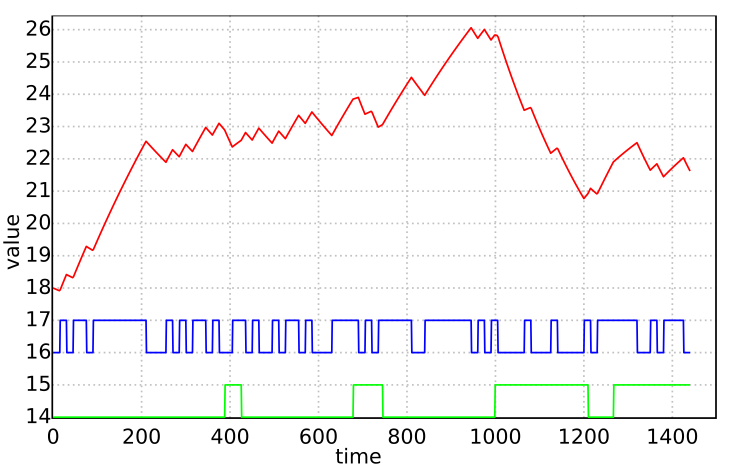
\includegraphics[width=\linewidth]{images/2_a.png}
            \caption{Stochastic, $D(24h)=4200$.} \label{fig:2a}
        \end{subfigure}%
        \hspace*{\fill}
        \begin{subfigure}{0.51\textwidth}
            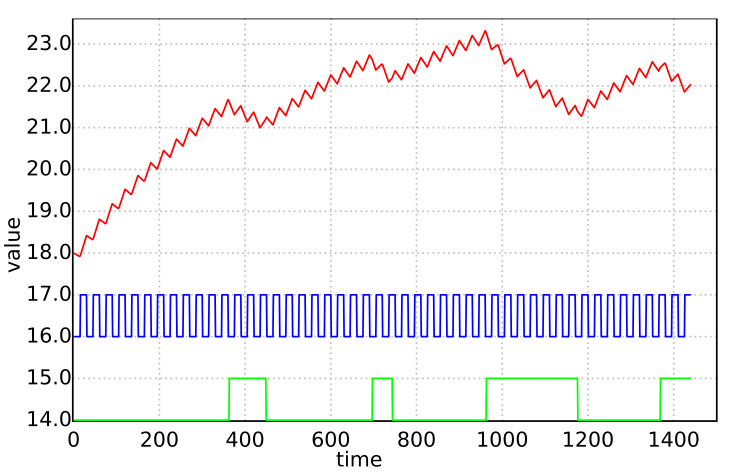
\includegraphics[width=\linewidth]{images/2_b.png}
            \caption{Offline naive. $D(24h)=2750$.} \label{fig:2b}
        \end{subfigure}%    
        \\
        \begin{subfigure}{0.51\textwidth}
            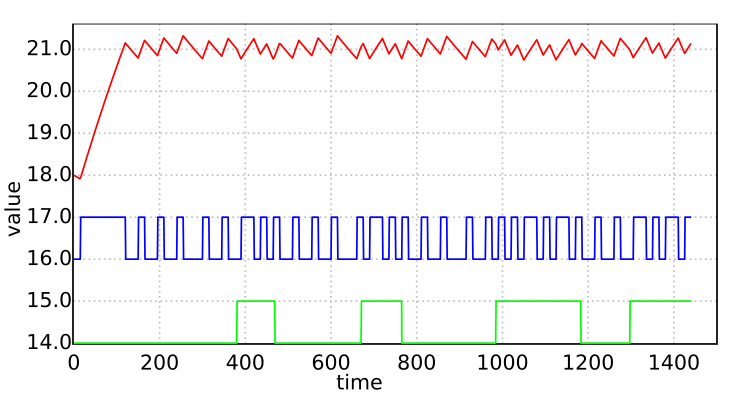
\includegraphics[width=\linewidth]{images/2_c.png}
            \caption{Offline splitting, $D(24h)=468$.} \label{fig:2c}
        \end{subfigure}%
        \hspace*{\fill} 
        \begin{subfigure}{0.51\textwidth}
            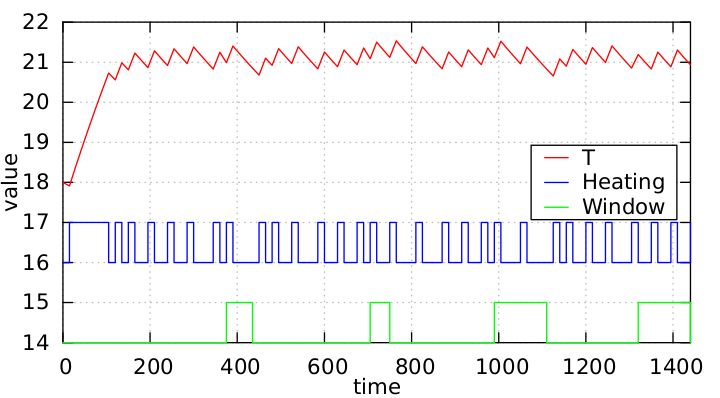
\includegraphics[width=\linewidth]{images/2_d.png}
            \caption{Online naive, $D(24h)=471.5$.} \label{fig:2d}
        \end{subfigure}%
        \caption{One-room 24h trajectories of various control strategies}
    \end{figure}

    \textbf{Online Synthesis}
    \textsc{Uppaal Stratego} [5,6] provides a method for aproximating 
    $\mathbb{E}^{\mathcal{G},\gamma}_{\sigma,H}(D) \in \mathbb{R}_{\geqslant 0}$
    by computing a near-optimal strategy $\sigma^H$ for a given horizon $H$ using 
    reinforcemente learning. However, the effort needed to learn the strategy 
    $\sigma^H$ with a desired precision and confidence-level grows exponentially
    in the number of dimensions (variables). The quality of the learned control 
    degrades sharply after the control options outnumber the number of simulation
    runs during learning, making this direct application of \textsc{Uppaal Stratego}
    limited in the time horizon. For instance, given a realistic setting of eleven 
    heating switches as considered in our case study, the controller is faced with  
    $2^11=2048$ distinct options at each 15min period and thus \textsc{Uppaal Stratego}
    manages to compute sensible heating configuration only for the first two periods 
    (yieldings $2048^2=4194304$ combinations in total) and then it simply resolves 
    to default option of no heating at all.
    Instead of learning --- at great computational expense -- the   entire strategy
    $\sigma^H$, we propose a method for attentively and online (i.e while playing
    the game \textsc{G} in the real setting) to compute a near-optimal strategy for 
    controllable mode-change at the next period. More precisely, the resulting online 
    and periodic strategy $\sigma^O$ will base the mode-change at time $nP$ not only
    on the configuration at that point ($\gamma_n$) but also on the configuration
    ($\gamma_{n-1}$) at time $(n-1)P$\footnote{Note that there way be several configurations
    between $\gamma_{n-1}$ and $\gamma_n$ due to the environment $\mathcal{U}$ changing
    the uncontrollable mode.}, which will be used as the basis for online
    learning of short-horizon $(h << H)$ strategies.

    \begin{table}[H]
    \caption{Performance evaluation of one room controller synthesis: offline-3(-6) methods
        synthetize strategy for entire 72 hours (144 hours respectively ) at once,
        strategy distance is evaluated on 70 simulations; online-3 methods synthetize
        a strategy for 5 periods of 15 min ahead and repeat synthesis and execution until 
        72 hours are covered, the distance is averaged over 70 online simulations.
    }


    \centering
    \begin{tabular}{|c|l|r|r|r|r|r|r|}
    \hline
    % \parbox[t]{2mm}{\multirow{2}{*}{Synthesis method}}
    & \multirow{2}{*}{ \textbf{\pbox{10cm}{Synthesis \\ method}} } & \multicolumn{3}{c|}{ \textbf{Purely dynamical model} } & \multicolumn{3}{c|}{ \textbf{Extra period counter} } \\
    % \hline
    & & \multicolumn{1}{c|}{ \textbf{Distance} } & \multicolumn{1}{c|}{ \textbf{cpu,s} } & \multicolumn{1}{c|}{ \textbf{mem,kB}} & \multicolumn{1}{c|}{ \textbf{Distance} } & \multicolumn{1}{c|}{ \textbf{cpu,s} } & \multicolumn{1}{c|}{ \textbf{mem,kB} } \\
    \hline
    \bfseries \parbox[t]{2mm}{\multirow{4}{*}{\rotatebox[origin=c]{90}{Offline-3}}}
    & naive & 10227.8 & 1555.15& 11884& 3671.84 & 566.4 & 9448 \\
    & splitting & 517.9 & 1640.06 & 13424& 2361.80 & 1608.48 & 90740\\
    & covariance & 10227.8 & 1298.66& 11896& 1091.81 & 1668.45 & 22820 \\
    & regression & 10227.8 & 1368.34 & 11480& 1387.84 & 1767.50 & 19196 \\
    \hline
    \bfseries \parbox[t]{2mm}{\multirow{4}{*}{\rotatebox[origin=c]{90}{Offline-6}}}
    & naive & 19668.8 & 1855.36 & 11836 & 8032.86 & 1316.08 & 20820\\
    & splitting & 593.7 & 3200.38 & 13112 & 8260.19 & 3120.03 & 167308 \\
    & covariance & 20234.3 & 2039.30 & 11528 & 2468.91 & 3258.09 & 39580 \\
    & regression & 19007.2 & 2525.13 & 12148 & 3425.62 &  3488.26 & 28416 \\
    \hline
    % ±
    \bfseries \parbox[t]{2mm}{\multirow{4}{*}{\rotatebox[origin=c]{90}{Online-3}}}
    & naive & 584.7$\pm$1.0 & 1046.5$\pm$5.0 & 7240 & 526.6$\pm$0.5 & 1227.1$\pm$3.2 & 7328 \\
    & splitting & 547.7$\pm$0.6 & 1136.4$\pm$3.6 & 7384 & 526.1$\pm$0.6 & 1240.8$\pm$2.5 & 7384 \\
    & covariance & 587.5$\pm$1.2 & 1084.0$\pm$3.9 & 7272 & 527.1$\pm$0.6 & 1158.5$\pm$2.5 & 7624 \\
    & regression & 585.3$\pm$1.0 & 1173.9$\pm$3.4 & 9052 & 527.9$\pm$0.5 & 1337.1$\pm$2.5 & 7380 \\
    \hline
    \end{tabular}
    \end{table}

    Formally:
    \begin{equation*}
        \sigma^O (\gamma_{n-1},\gamma_{n}) = \text{def } \textbf{let}(\sigma^h = \textbf{argmin}_{\sigma}\mathbb{E}^{\mathcal{G},\gamma_{n-1}}_{\sigma,h}(D) ) \textbf{ in } \sigma^h(\gamma_n) 
    \end{equation*}

    We leave the formal definition of runs under the one-step-memory strategy $\sigma^O$
    to the reader (slightly more complicated version of runs under a memoryless strategy given above).
    However, we note that $\sigma^O$ may be used for an arbitrary finite horizon $H$ or 
    even as a strategy of infinite horizon. To maximize the quality of $\sigma^O$, the choice
    of the small horizon $h$ should be such that it just allows the learning of $\sigma^h$
    to be completed between the two configurations $\gamma_{n-1}$ and $\gamma_n$, i.e.
    within the period $P$.

    \clearpage


\section{Safe and near optimal controller for sthocastic hybrid games}
    \textbf{Model Predictive Control} 
    In principle, model predictive control is very effective in discrete control.
    Now consider the issue of critical systems where is mandatory a safe evolve 
    along the control. This suggest to incorporate a sequence of modes that guarantee
    a safe system. For this reason the study incorporat e a methodology to find patterns
    for non linear hybrid systems [ref adrien].
    \clearpage
